% =========================================================================
% CAPITOLO 2 — DOMANDE DI RICERCA E OBIETTIVI
% =========================================================================

\chapter{Domande di ricerca e obiettivi}
\label{ch:rqs}

\noindent
{\rmfamily\itshape
\begin{tabular}[t]{@{}l@{\hspace{0.3cm}}p{12.5cm}@{}}
\textls[50]{\textbf{Trattati:}} &
\textls[50]{Domande di ricerca chiave · Questioni da affrontare · Assunzioni da validare ·
Obiettivi del progetto · Ipotesi e proposizioni progettuali · Matrice di allineamento · Disciplina dell'ambito}
\end{tabular}
}

\vspace{0.5cm}

% -------------------------------------------------------------------------
\section{Quadro della ricerca}
\label{sec:rq-framework}

Il Capitolo~\ref{ch:introduction} ha individuato un problema di rappresentazione: i sistemi climatici complessi a rischio di tipping restano cognitivamente fuori portata per i non specialisti anche quando i dati sono aperti e leggibili. Questo capitolo formalizza il programma che lo affronta, seguendo l'arco in tre fasi di \emph{rilevare, tradurre e valutare}, adattato dalla ricerca basata sul design nelle scienze dell'apprendimento, dove progettare una soluzione è esso stesso trattato come ricerca \citep{andersonshattuck2012, barab2004}. Le fasi sono collegate: ciò che si rileva fissa ciò che si può tradurre, e ciò che si traduce diventa ciò che si valuta. Un'unica domanda di ricerca centrale le connette, e tre sotto-domande --- una per fase --- la indagano attraverso tipi diversi di evidenza.

Le tre fasi non pesano allo stesso modo.\footnote{La fase di \emph{rilevamento} è analitica ed è riportata per esteso; la fase di \emph{valutazione} è esplorativa e offre una valutazione iniziale anziché una validazione definitiva.} Il baricentro è il ponte tra le prime due: tradurre la struttura ricavata dal machine learning in rappresentazioni costruite per migliorare la comprensione. Quel ponte è il contributo metodologico originale; la valutazione si chiede se sia promettente.

% -------------------------------------------------------------------------
\section{Domande di ricerca}
\label{sec:rqs}

La domanda centrale guida la tesi nel suo insieme, ed è deliberatamente valutativa anziché meramente orientata al design:

\begin{quote}
\textbf{RQ.} \emph{In che misura le visualizzazioni esperienziali guidate dal machine learning migliorano la comprensione cognitiva dei sistemi climatici complessi a rischio di tipping tra il pubblico non specialista, rispetto alle visualizzazioni statiche convenzionali?}
\end{quote}

Ogni elemento è una scelta. \emph{In che misura\ldots rispetto a} fissa una cornice comparativa: lo scopo non è costruire una visualizzazione ma verificare se sostenga la comprensione meglio di una convenzionale. \emph{Pubblico non specialista} indica partecipanti caratterizzati dal background, non un pubblico indefinito; \emph{sistemi climatici complessi a rischio di tipping} indica la classe di processi di cui l'AMOC è il caso. La tesi non si chiede se il machine learning possa predire un punto di tipping dell'AMOC --- questione ancora dibattuta \citep{benyami2024, ditlevsen2023} --- ma se la struttura latente che recupera possa essere tradotta in rappresentazioni che aiutano i non specialisti a comprendere un sistema altrimenti invisibile.

Tre sotto-domande seguono le tre fasi:

\begin{quote}
\textbf{RQ1} (analitica). \emph{Quali pattern strutturali latenti e firme dinamiche della variabilità dell'AMOC può recuperare il machine learning dal record RAPID e dall'ensemble di rianalisi Copernicus; con quanta fedeltà preservano la dinamica sottostante, e un autoencoder non lineare recupera qualche struttura che la decomposizione lineare non coglie; e sono abbastanza interpretabili da fungere da substrato per una rappresentazione destinata ai non specialisti?}
\end{quote}

RQ1 è descrittiva ed esplorativa, modesta su ciò che promette: non un nuovo risultato sull'oceano ma un resoconto onesto di ciò che il record contiene. La parola che porta il peso è \emph{fedeltà} --- applicare un metodo non prova nulla; ciò che conta è che la versione a bassa dimensionalità mantenga la struttura del sistema che rappresenta, l'unico terreno su cui costruire il resto della tesi.

\begin{quote}
\textbf{RQ2} (progettuale). \emph{Come possono le strutture latenti di RQ1 essere tradotte in rappresentazioni interattive ed esperienziali che comunichino le dinamiche dell'AMOC, la sua invisibilità e il rischio di tipping, fondate sulla cognizione incarnata e sulla visualizzazione delle informazioni?}
\end{quote}

RQ2 è generativa: non ha un'unica risposta corretta, solo una gamma di risposte che possono essere costruite e difese. Ciò che produce è l'insieme di rappresentazioni che RQ3 verifica --- non il punto d'arrivo della tesi, ma ciò che essa esamina.

\begin{quote}
\textbf{RQ3} (empirica). \emph{In che misura le rappresentazioni dinamiche ed esperienziali delle dinamiche dell'AMOC, rispetto a una convenzionale statica, sostengono il modo in cui il pubblico non specialista sviluppa ed esprime la propria comprensione del comportamento di un sistema complesso?}
\end{quote}

RQ3 è comparativa ma esplorativa: osserva come i partecipanti descrivono e organizzano la propria comprensione sotto l'una o l'altra rappresentazione, anziché misurare l'efficacia su scala di popolazione. Nessuna sotto-domanda risponde da sola a quella centrale: RQ1 trova la struttura, RQ2 costruisce la rappresentazione, RQ3 la verifica rispetto alla baseline.

% -------------------------------------------------------------------------
\section{Obiettivi}
\label{sec:objectives}

Ciascuna sotto-domanda diventa un insieme di obiettivi con output definiti, legati nella matrice di allineamento (Tabella~\ref{tab:alignment}) al capitolo che li realizza e all'affermazione che fanno avanzare. Letta per colonne, quella matrice mostra tre programmi coerenti --- analitico, progettuale, empirico; letta per righe, mostra come ogni fase alimenti la successiva. Funziona come un contratto promissorio: per ogni impegno preso qui, una consegna localizzabile in un capitolo successivo.

Gli obiettivi analitici strutturano il Capitolo~\ref{ch:data_pipeline}: recuperare la struttura verticale latente tramite analisi delle componenti principali (\textbf{O1.1}), verificare se quella struttura sia genuinamente a bassa dimensionalità rispetto a un autoencoder non lineare a dimensionalità pari (\textbf{O1.2}), caratterizzare le anomalie del record e testare i segnali di preallarme sotto un test di significatività corretto (\textbf{O1.3}), e segnare come fuori ambito un livello di previsione probabilistica (\textbf{O1.4}).

Gli obiettivi progettuali strutturano il Capitolo~\ref{ch:translate}: definire le condizioni di rappresentazione su informazione condivisa (\textbf{O2.1}), sviluppare la grammatica di design trasferibile che mappa le feature del machine learning sui canali percettivi (\textbf{O2.2}), e codificare il mutevole disaccordo tra ricostruzioni come qualità percettiva sentita anziché come annotazione numerica (\textbf{O2.3}).

Gli obiettivi empirici strutturano i Capitoli~\ref{ch:userstudy} e~\ref{ch:results}: costruire lo strumento (\textbf{O3.1}), condurre lo studio a due gruppi (\textbf{O3.2}), e valutare se le codifiche percettive siano lette come inteso (\textbf{O3.3}).

% -------------------------------------------------------------------------
\section{Ipotesi e proposizioni progettuali}
\label{sec:hypotheses}

Le sotto-domande differiscono per natura, perciò le affermazioni sono formulate di conseguenza: RQ1 ammette \emph{ipotesi} direzionali; RQ2 avanza \emph{proposizioni progettuali} valutate rispetto a criteri di design; RQ3 enuncia \emph{aspettative} esplorative. Trattarle come equivalenti travisarebbe l'evidenza che ciascuna può portare \citep{cronbach1975, mckenney2018}. Due ipotesi ombrello inquadrano il tutto: che le rappresentazioni statiche convenzionali siano insufficienti per i non specialisti, presentando la complessità come informazione da leggere anziché come processo da cogliere (\textbf{H-A}); e che le rappresentazioni derivate dal machine learning, rese dinamiche ed esperienziali, possano cambiare il modo in cui i non specialisti comprendono il comportamento del sistema rendendone percepibile la struttura, non sostituendo l'analisi (\textbf{H-B}).

Le ipotesi analitiche sono direzionali e riportate nel Capitolo~\ref{ch:data_pipeline}. \textbf{H1}: pochi modi lineari --- due o tre --- spiegano gran parte della varianza (qui presa come superiore all'\SI{80}{\percent}) nei profili verticali dell'AMOC \citep{buckley2016, hannachi2007}. \textbf{H2}: un autoencoder non lineare non supera in modo sostanziale la PCA a dimensionalità pari, perciò coordinate lineari interpretabili perdono poco \citep{baldi1989}. \textbf{H3}: una volta corretta la dimensione campionaria effettiva per l'autocorrelazione nelle finestre sovrapposte, i segnali di preallarme classici non mostrano alcun trend significativo lungo il record RAPID.\footnote{H3 è deliberatamente formulata attorno a un risultato nullo. Mostrare che un segnale apparente scompare una volta trattata correttamente la dipendenza statistica non è un fallimento ma una dimostrazione di robustezza metodologica \citep{dakos2012, scheffer2009}.}

Le proposizioni progettuali sono realizzate nel Capitolo~\ref{ch:translate}. \textbf{DP2.1}: le feature del machine learning --- posizione latente, punteggio di anomalia, incertezza d'ensemble --- possono essere mappate su dimensioni percettive quali colore, movimento, densità e suono, in modo coerente con l'elaborazione pre-attentiva e la cognizione incarnata \citep{lakoff1999, ware2021}. \textbf{DP2.2}: il mutevole disaccordo tra ricostruzioni indipendenti della stessa quantità può essere codificato come variazione percettiva sentita anziché come annotazione numerica.

Le aspettative empiriche guidano l'analisi qualitativa. \textbf{E3.1}: il gruppo sperimentale descriverà il comportamento dell'AMOC --- le sue dinamiche, la non linearità, l'invisibilità --- in modi qualitativamente diversi dal gruppo di controllo, indipendentemente dal fatto che ciò corrisponda a guadagni misurabili nella prova di comprensione. \textbf{E3.2}: le codifiche percettive introdotte dalla condizione esperienziale --- l'incertezza tra queste --- produrranno interpretazioni che il questionario e l'analisi possono far emergere, indipendentemente dal fatto che tali interpretazioni corrispondano alla lettura intesa; e la fiducia in una lettura non seguirà in modo affidabile la sua correttezza \citep{fischer2020}. Nessuna delle due aspettative presume una direzione o un'entità dell'effetto.

% it/figures/research_questions/rq_tree.tex — versione italiana
\begin{figure}[!ht]
    \centering
    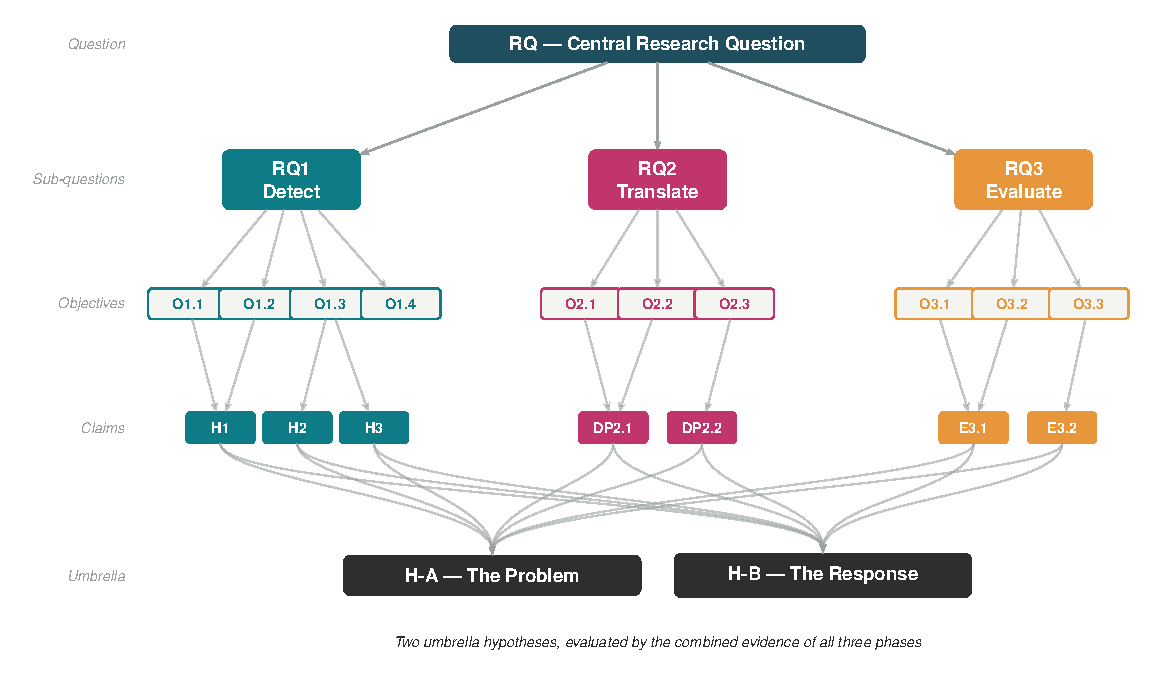
\includegraphics[width=\textwidth]{figures/research_questions/rq_tree_preview.pdf}
    \caption[Struttura delle domande di ricerca, degli obiettivi, delle affermazioni e delle ipotesi ombrello.]{\textbf{L'architettura
    del programma di ricerca.} La domanda di ricerca centrale si dirama in tre
    sotto-domande lungo l'arco rilevare--tradurre--valutare. Ogni sotto-domanda genera
    i propri obiettivi (O1.1--O1.4, O2.1--O2.3, O3.1--O3.3), che danno luogo alle
    affermazioni appropriate al loro carattere epistemico: ipotesi direzionali
    (H1--H3), proposizioni di design (DP2.1--DP2.2) e aspettative empiriche
    (E3.1--E3.2). Tutti e tre i gruppi di affermazioni convergono sulle due ipotesi
    ombrello, H-A (il problema) e H-B (la risposta), valutate non da un singolo
    strumento ma dall'evidenza combinata dell'intero programma.}
    \label{fig:rq-tree}
\end{figure}


% -------------------------------------------------------------------------
\section{Fattibilità e disciplina dell'ambito}
\label{sec:rq-feasibility}

La fattibilità poggiava su infrastruttura, tempo e controllo dell'ambito. La fase analitica ha attinto al record RAPID e all'ensemble Copernicus, elaborati e riportati nel Capitolo~\ref{ch:data_pipeline}, realizzando O1.1--O1.3, con O1.4 lasciato come confine di ambito. La fase empirica ha richiesto una preparazione modesta: un questionario di venti minuti somministrato a venticinque partecipanti non specialisti, assegnati casualmente a due gruppi --- una condizione statica convenzionale come controllo e una condizione esperienziale costruita su visualizzazioni interattive guidate dal machine learning. Un campione di queste dimensioni si addice a uno studio esplorativo di primo stadio volto a individuare pattern iniziali nel modo in cui i partecipanti comprendono il sistema, anziché sostenere un'inferenza su scala di popolazione statisticamente potente \citep{braunclarke2006, smithmcgannon2018, malterud2016}. La fase di design è stata la principale impresa tecnica, sviluppata lungo i Capitoli~\ref{ch:methodology} e~\ref{ch:translate}.

Il tempo è stato il vincolo principale, perciò la parte più rischiosa --- costruire la condizione esperienziale --- è avvenuta una volta assestato il testo circostante. Mantenere l'ambito ristretto è stata una scelta metodologica: la previsione è stata lasciata da parte per tenere la tesi sulla rappresentazione anziché sulla predizione \citep{sonnewald2021}, il prototipo è rimasto un artefatto di ricerca, e lo studio è rimasto principalmente esplorativo. Due piani di riserva hanno mantenuto coerente la tesi: se lo studio fosse andato in ritardo, i capitoli analitici e di design sarebbero stati autosufficienti; e se la costruzione fosse fallita, la grammatica di design avrebbe comunque contato come contributo (O2.2). La tesi è ambiziosa ma focalizzata --- ogni obiettivo commisurato al tempo disponibile, ogni affermazione all'evidenza che può reggere.

\begin{table}[!ht]
    \centering
    \small
    \setlength{\tabcolsep}{5pt}
    \renewcommand{\arraystretch}{1.25}
    \caption{Allineamento tra le tre sotto-domande e la struttura operativa della tesi, incluso come ciascuna è validata e rispetto a quale criterio.}
    \label{tab:alignment}
    \begin{tabular}{
        @{}
        >{\RaggedRight\arraybackslash}p{2.7cm}
        >{\RaggedRight\arraybackslash}p{3.7cm}
        >{\RaggedRight\arraybackslash}p{3.7cm}
        >{\RaggedRight\arraybackslash}p{3.7cm}
        @{}
    }
        \toprule
        & \textbf{RQ1 --- Rilevare}
        & \textbf{RQ2 --- Tradurre}
        & \textbf{RQ3 --- Valutare} \\
        \midrule
        \makecell[l]{\textbf{Carattere}\\\textbf{epistemico}}
            & Analitico, comparativo, esplorativo
            & Progettuale, generativo
            & Empirico, qualitativo, comparativo \\[0.5em]

        \textbf{Capitoli}
            & Cap.~\ref{ch:background}, Cap.~\ref{ch:data_pipeline}
            & Cap.~\ref{ch:methodology}, Cap.~\ref{ch:translate}
            & Cap.~\ref{ch:methodology}, Cap.~\ref{ch:userstudy}, Cap.~\ref{ch:results} \\[0.5em]

        \textbf{Obiettivi}
            & O1.1--O1.4
            & O2.1--O2.3
            & O3.1--O3.3 \\[0.5em]

        \textbf{Affermazioni}
            & H1, H2, H3
            & DP2.1, DP2.2
            & E3.1, E3.2 \\[0.5em]

        \textbf{Materiale}
            & Osservazioni RAPID, ensemble di rianalisi Copernicus
            & Strutture latenti recuperate in RQ1
            & Condizioni prodotte in RQ2; partecipanti non specialisti \\[0.5em]

        \makecell[l]{\textbf{Metodo di}\\\textbf{validazione}}
            & Analisi comparativa dei modelli: PCA vs.\ autoencoder a dimensionalità pari; EWS con correzione per pseudo-replicazione; Isolation Forest
            & Costruzione design-science rispetto alla grammatica (Tabella~\ref{tab:design-grammar}); audit di provenienza condivisa della provenienza allineata
            & Studio tra soggetti, venticinque partecipanti non specialisti (dodici controllo, tredici sperimentale), assegnati casualmente alle condizioni statica di controllo ed esperienziale interattiva guidata dal ML; valutazione tramite questionario e analisi esplorativa \\[0.5em]

        \makecell[l]{\textbf{Criterio di}\\\textbf{successo}}
            & Scarto latente $\leq$ errore di ricostruzione; trend nullo correttamente identificato, non forzato
            & Ogni valore a schermo tracciabile al bundle; condizioni equivalenti per costruzione della provenienza
            & Il gruppo sperimentale articola struttura che il gruppo di controllo non articola, nella descrizione spontanea --- valutato per scena, poiché il criterio può essere soddisfatto per alcune strutture e non per altre \\[0.5em]

        \textbf{Output}
            & Analisi della struttura latente; risultato nullo EWS; caratterizzazione delle anomalie
            & Tre condizioni di rappresentazione; grammatica di design documentata
            & Risposte anonimizzate; analisi deduttiva a codebook rispetto a una griglia definita a priori; confronto descrittivo tra i due gruppi \\[0.5em]

        \textbf{Ancoraggio SDG}
            & 13 (Lotta al cambiamento climatico), 14 (La vita sott'acqua)
            & 4 (Istruzione di qualità), 13
            & 4, 13 \\[0.5em]

        \makecell[l]{\textbf{Disciplina}\\\textbf{dell'ambito}}
            & Previsione LSTM rinviata a lavori futuri
            & Prototipo di ricerca, non artefatto di produzione
            & Confronto esplorativo a due gruppi; prevalentemente qualitativo, non statisticamente potente \\
        \bottomrule
    \end{tabular}
\end{table}
